One can define the relationship between the tasks as follows, in figure \ref{fig:GwOverview}. The rule of the gateway is to receive LoRa messages and send the content in TCP-IP messages, or vice versa.

\begin{figure}[H]
	\centering
	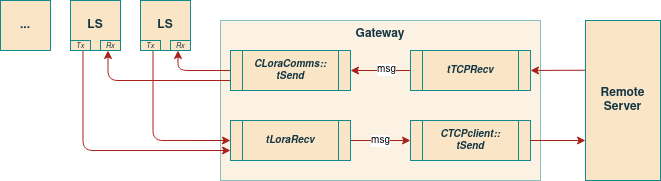
\includegraphics[width=1\textwidth]{09sw_specification/Gateway/overview}
	\caption{Gateway Overview.}
	\label{fig:GwOverview}
\end{figure}

%**********************************************************
\subsection{Class Diagrams}
In figure \ref{fig:GwclassDiag} is represented the class diagram of gateway, \textit{CGateway}, which is the main class of the system, responsible for initializing the objects of each class listed below.

\begin{itemize}
	\item \textbf{CLoraComm:} manages the LoRa communications with the local systems, interfacing with the LoRa module; this class was already detailed previously;
	
	\item \textbf{CTCPclient:} manages the TCP-IP communication with the remote server;
\end{itemize}

\begin{figure}[H]
	\centering	\includegraphics[width=.68\textwidth]{09sw_specification/Gateway/cgateway/class}
	\caption{CGateway Class Diagram.}
	\label{fig:GwclassDiag}
\end{figure}

\myparagraph{Class CTCPclient}

In figure \ref{fig:TCPclientClass} is shown the CTCPclient class. This class defines a TCPclient capable of establishing a connection to a given remote server and to exchange messages to it, via TCP-IP. Like in the CLoraComm class, this class inherits from the class CCommunication.

\begin{figure}[H]
	\centering
	\includegraphics[width=.4\textwidth]{09sw_specification/Gateway/ctcpclient/class}
	\caption{Class Diagram: TCPclient.}
	\label{fig:TCPclientClass}
\end{figure}

%**********************************************************
\clearpage
\subsection{Task Overview}
One can define and describe briefly how the gateway is implemented, making use of threads and processes.

\begin{itemize}
	\item \textbf{CGateway::tLoraRecv:} receives all messages from local systems, using LoRa communication;
	\item \textbf{CGateway::tTCPRecv:} receives all messages from the remote server, using TCP-IP communication;	
	\item \textbf{CLoraComm::tSend:} sends all received messages from the remote server, in \textit{tTCPRecv}, to the local systems, using LoRa communication; 
	\item \textbf{CTCPclient::tSend:} sends all received messages from local systems, in \textit{tLoraRecv}, to the remote server, using TCP-IP communication;
\end{itemize}

%**********************************************************
\subsection{Task Priority}
The priority assignment diagram for the gateway is represented in figure \ref{fig:gwt_priority}.

\begin{figure}[H]
	\centering
	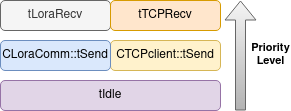
\includegraphics[width=0.6\textwidth]{09sw_specification/Gateway/priority}
	\caption{Gateway Priority Assignment Schematic.}
	\label{fig:gwt_priority}
\end{figure}

%**********************************************************
\subsection{Task Synchronization}

\myparagraph{Condition Variables}

The condition variables used in this system are listed below.

\begin{itemize}
	\item \textbf{CCommunication::condSend:} already detailed in the local system section; this condition variable is used indirectly by \textit{CTCPclient} and \textit{CLoraComm}.
\end{itemize}

\myparagraph{Mutexes}

The mutexes used in this system are listed below.

\begin{itemize}
	\item \textbf{CCommunication::mutComms} and \textbf{CCommunication::mutTxMsgs:} already detailed in the local system section; this mutexes are used indirectly by \textit{CTCPclient} and \textit{CLoraComm}.
\end{itemize}

%%**********************************************************
\subsection{Start-up Process}
In figure \ref{fig:bootGateway} is shown the start-up process for the gateway. When booting up, the gateway creates a CGateway object, initializing all needed members, and after that, runs until all the threads termination.

\begin{figure}[H]
	\centering		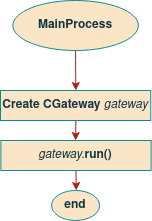
\includegraphics[width=.3\textwidth]{09sw_specification/Gateway/mainprocess}
	\caption{Start-Up Process: Gateway.}
	\label{fig:bootGateway}
\end{figure}

%**********************************************************
\clearpage
\subsection{Flowcharts}
%Each local system has a predefined ID, which may be presented in a physical label for an operator to use this information. When a local system is being installed, it will use it's predefined ID in all communications with the remote server until the operator registers the local system that's being installed, in the remote server. By doing this, the remote server assigns a new ID to the local system, which is then sent to the local system, for this to be used in further communications.

%*****************************
\myparagraph{CGateway Methods}

In figure \ref{fig:gwtCGatewayconstructor} is shown the \textit{CGateway} class constructor. With this, one can create a CTCPclient and a CLoraComm objects. After this the threads are created and both objects begin running their threads for receiving and sending messages.

\begin{figure}[H]
	\centering
	\includegraphics[width=.3\textwidth]{09sw_specification/Gateway/cgateway/constructor}
	\caption{Flowchart: CGateway constructor.}
	\label{fig:gwtCGatewayconstructor}
\end{figure}

\clearpage
This task, presented in figure \ref{fig:gwtLoraRecv}, is responsible for receiving all the packets sent by the local systems, through LoRa communication. When a message is received it is pushed into the TCP client list of queued messages, waiting to be sent to the remote server.

\begin{figure}[H]
	\centering
	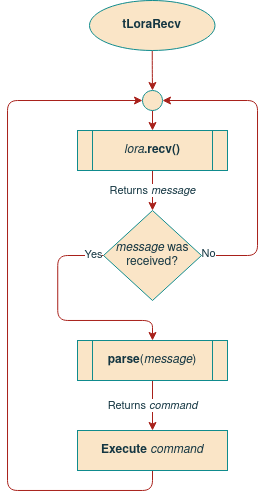
\includegraphics[width=.5\textwidth]{09sw_specification/Gateway/cgateway/tlorarecv}
	\caption{Flowchart: CGateway tLoraRecv method.}
	\label{fig:gwtLoraRecv}
\end{figure}

\clearpage
This task, presented in figure \ref{fig:gwtTCPRecv}, is responsible for receiving the messages sent by the remote system to the local systems. Unlike the \textit{tsend} tasks, this thread never enters the sleep state because one can receive a message at any moment. If it is received a message, then one can push the message to the messages queue in CLoraComm, signaling its thread to send the message, via LoRa communication.

\begin{figure}[H]
	\centering
	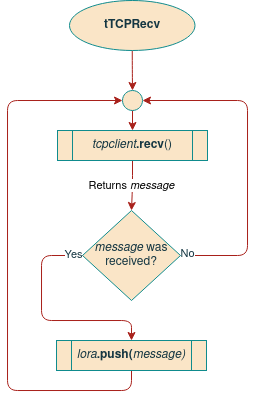
\includegraphics[width=.5\textwidth]{09sw_specification/Gateway/cgateway/ttcprecv}
	\caption{Flowchart: CGateway tTCPRecv method.}
	\label{fig:gwtTCPRecv}
\end{figure}

%*****************************
\clearpage
\myparagraph{CTCPclient Methods}

A TCPclient can be created through the use of the constructor, shown in figure \ref{fig:TCPclientconstructor}. This connects to a given server, defined by the string \textit{host}, and to the port \textit{port}, via TCP-IP and initializes all the private members.

\begin{figure}[H]
	\centering
	\includegraphics[width=.36\textwidth]{09sw_specification/Gateway/ctcpclient/constructor}
	\caption{Class Diagram: CTCPclient constructor.}
	\label{fig:TCPclientconstructor}
\end{figure}

As in CLoraComm, this class must implement \textit{recvFunc} and \textit{sendFunc}, as they are pure virtual methods from CCommunication. 

In this class, one will use existent functions \textit{TCPReceive} and \textit{TCPSend} to implement TCP-IP communication, as shown in figures \ref{fig:TCPclientrecvfunc} and \ref{fig:TCPclientsendfunc}. This functions make use of the socket created when the TCP-IP connection was established.

\begin{figure}[H]
	\centering
	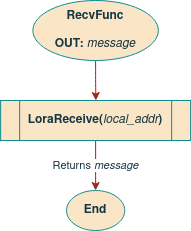
\includegraphics[width=.35\textwidth]{09sw_specification/Gateway/ctcpclient/recvfunc}
	\caption{Flowchart: CTCPclient recvFunc method.}
	\label{fig:TCPclientrecvfunc}
\end{figure}

\begin{figure}[H]
	\centering
	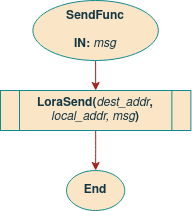
\includegraphics[width=.35\textwidth]{09sw_specification/Gateway/ctcpclient/sendfunc}
	\caption{Flowchart: CTCPclient sendFunc method.}
	\label{fig:TCPclientsendfunc}
\end{figure}

%**********************************************************
\clearpage
\subsection{Test Cases}
It is important to know how the gateway works, and how it will behave upon certain events. In table \ref{table:test_gateway} are shown test cases to this system.

\begin{table}[H]
	\centering
	\begin{threeparttable}
	\resizebox{\columnwidth}{!}
	{
		\begin{tabular}{|m{4cm}|m{5cm}||m{5cm}|}
			\hline
			\textbf{Test Case} & \textbf{Expected Output} & \textbf{Real Output}
			\\\hline\hline
			\multicolumn{3}{c}{\textbf{LoRa Communications}}\\\hline
			Establish connection with LS & Connection established & -
			\\\hline
			Receive message from LS & Identify the referent LS & -
			\\\hline
			Send message to a specific LS & Only the defined LS receives the message & -
			\\\hline
			Send message to a group of LS & All in the group receive the message & - 
			\\\hline
			
			\multicolumn{3}{c}{\textbf{TCP-IP Communications}}\\\hline
			Establish connection with RS & Connection established & -
			\\\hline
			Receive message from RS & Identify destination ID & -
			\\\hline
			Send message to the RS & Message sent & -
			\\\hline
		\end{tabular}
	}
	\begin{tablenotes}
		\small
		\item[LS]Local System
		\item[RS]Remote Server
	\end{tablenotes}
	
\end{threeparttable}	
	\caption{Test Cases: Gateway.}
	\label{table:test_gateway}
\end{table}
